\chapter{Anexo B}

%%pruebas con 5 nodos
\begin{figure}[!ht]
\centering
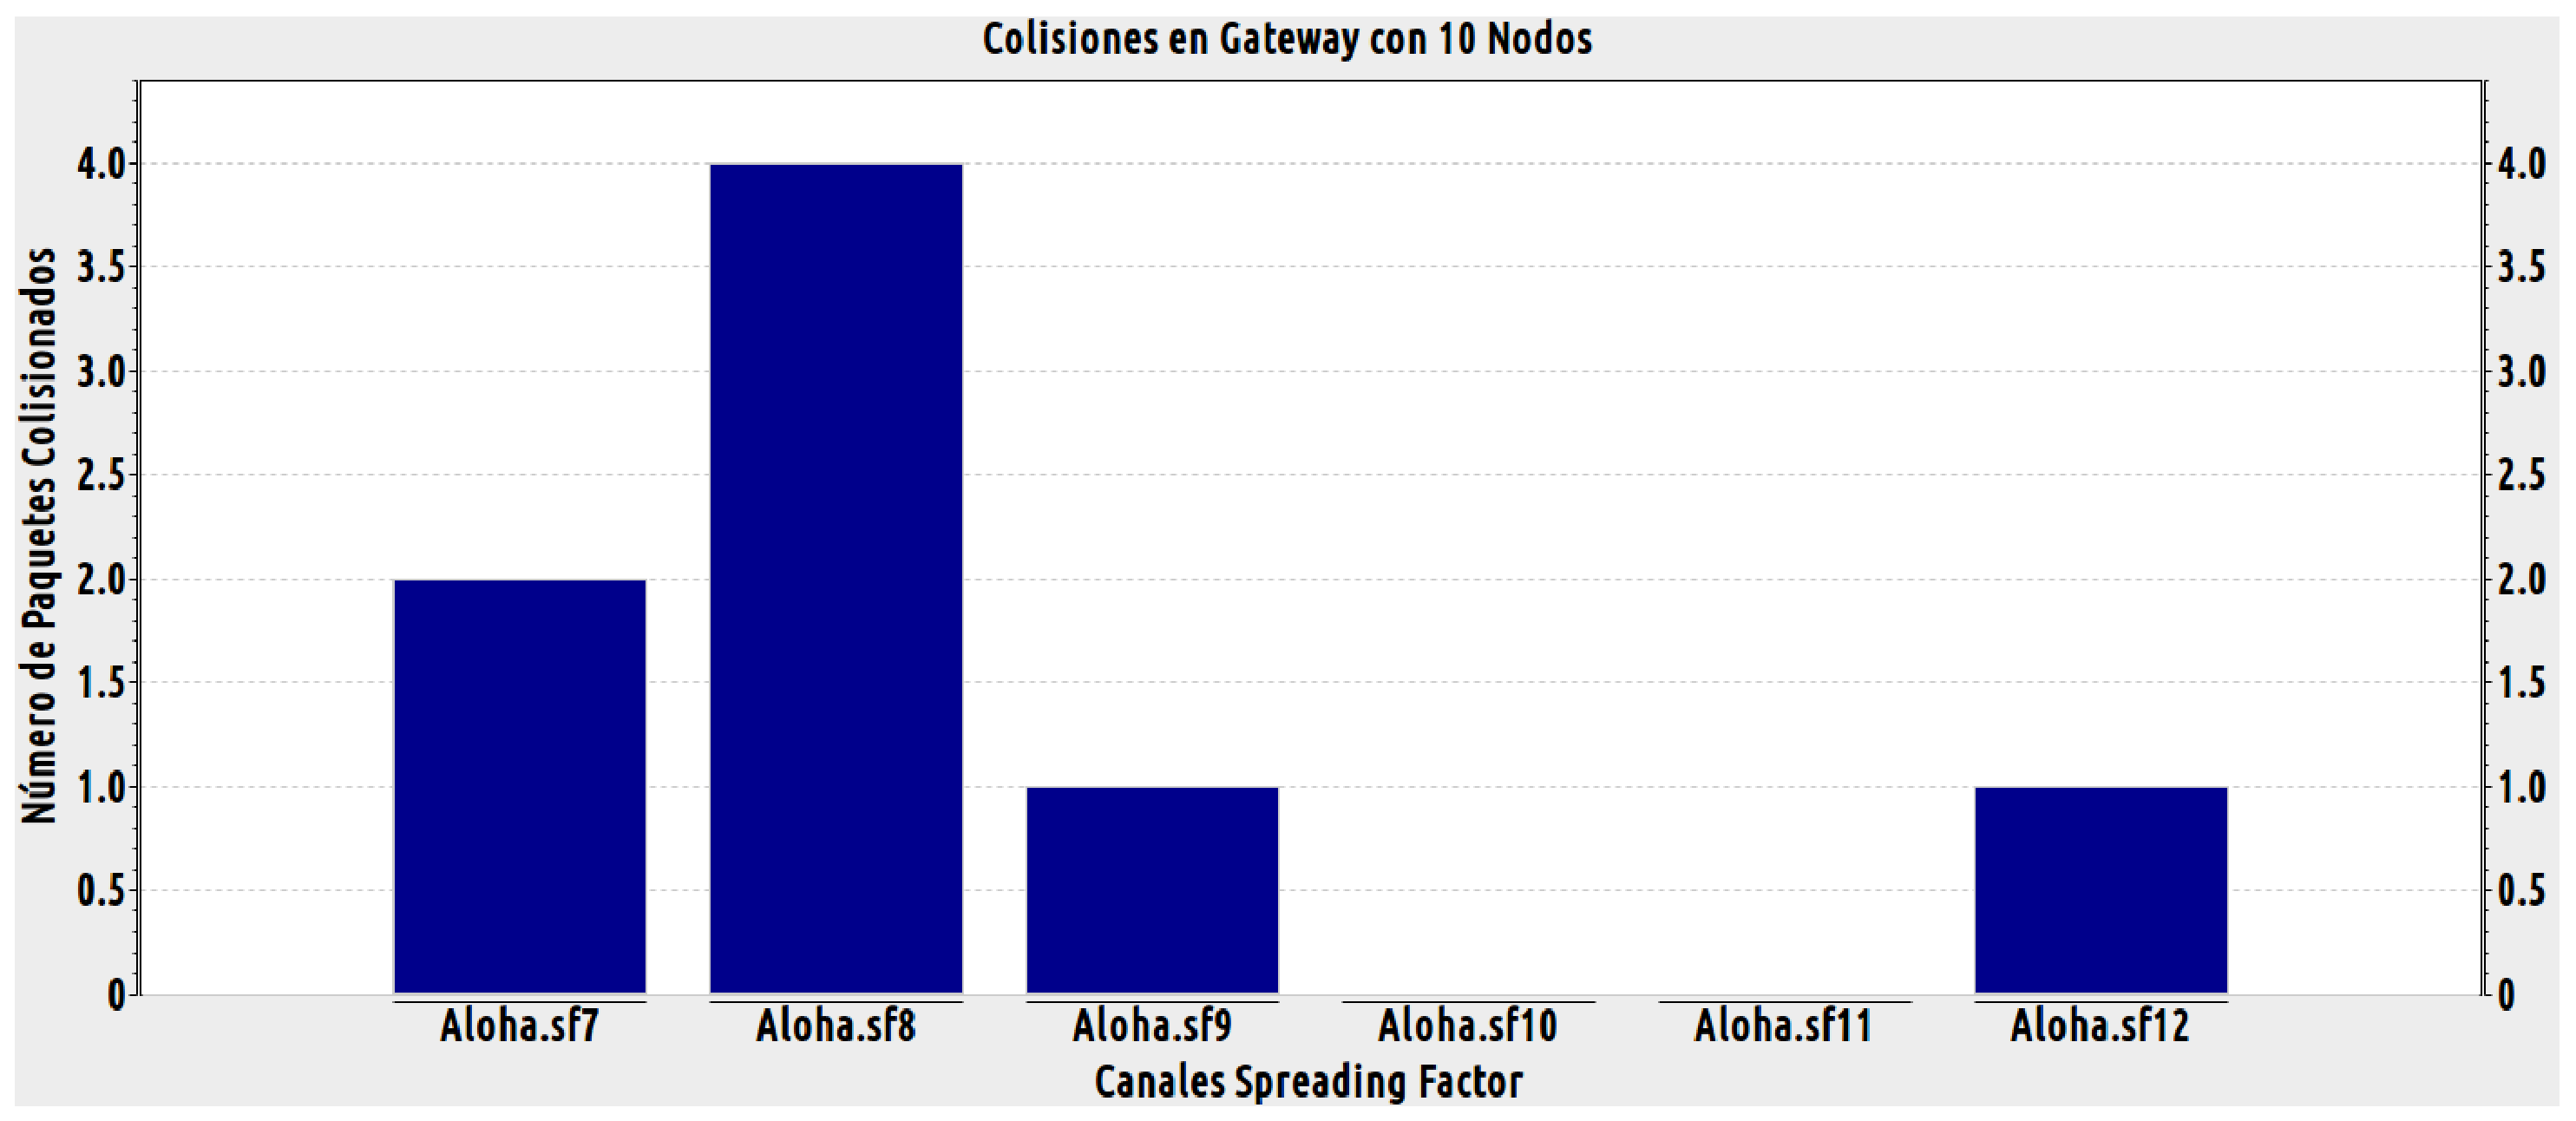
\includegraphics[angle=270, scale=0.4]{images/colisiones10nodos.eps}
\caption{Gráfico de colisiones ocurridos entre los distintos Spreading Factor, para 10 nodos transmitiendo}
\label{anexb:1}
\end{figure}


\begin{figure}[!ht]
\centering
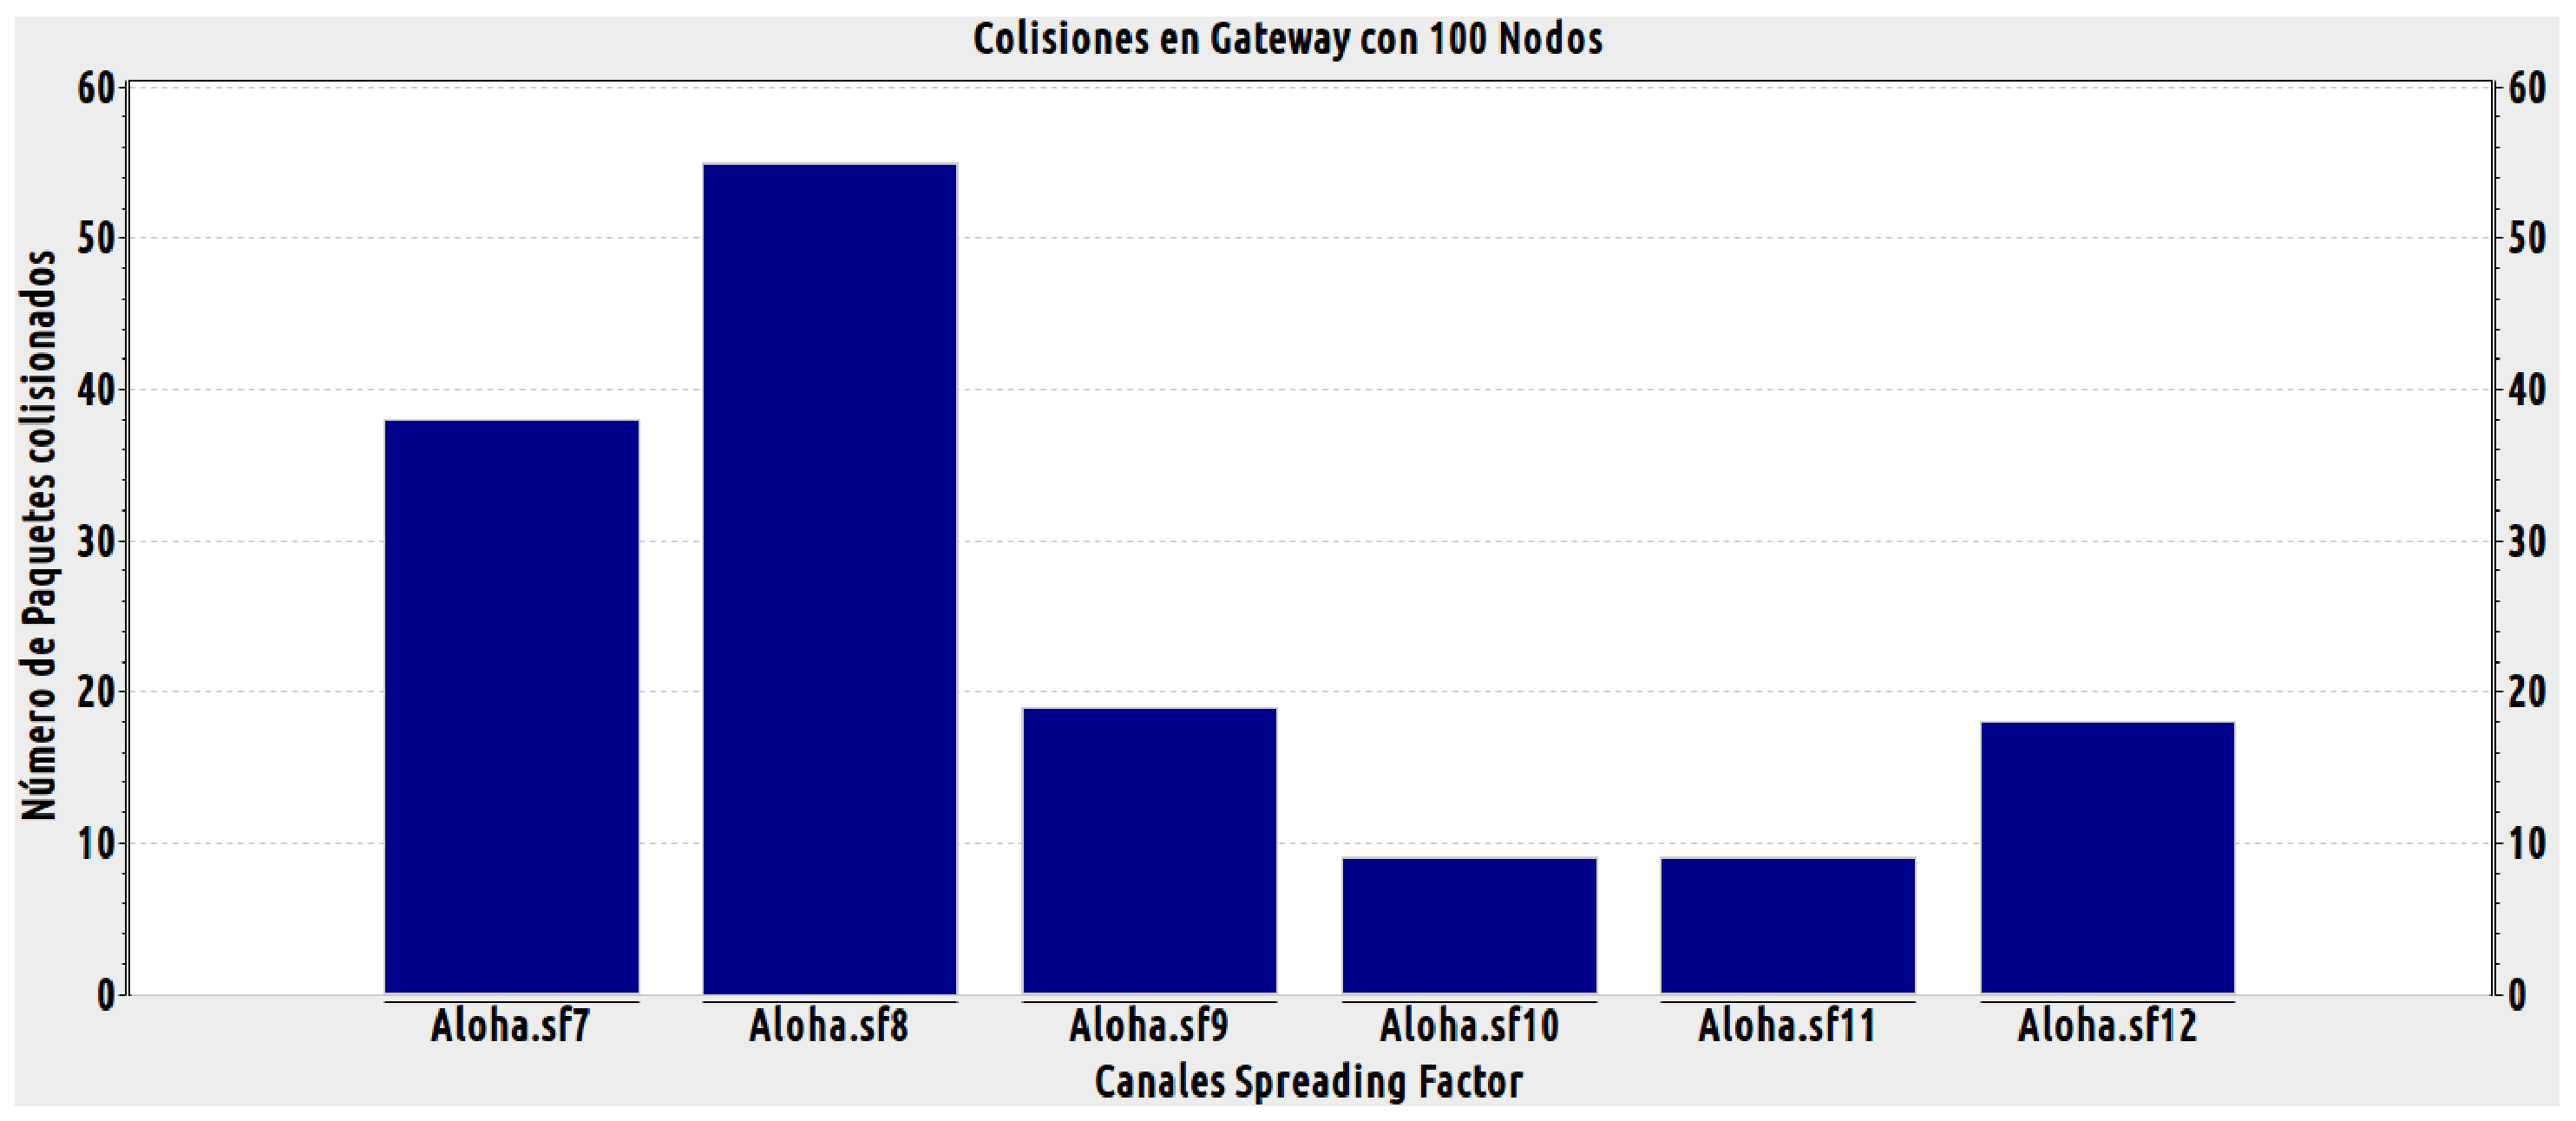
\includegraphics[angle=270, scale=0.4]{images/colisiones100nodos.eps}
\caption{Gráfico de colisiones ocurridos entre los distintos Spreading Factor, para 100 nodos transmitiendo}
\label{anexb:2}
\end{figure}

%% pruebas con 50 nodos
\begin{figure}[!ht]
\centering
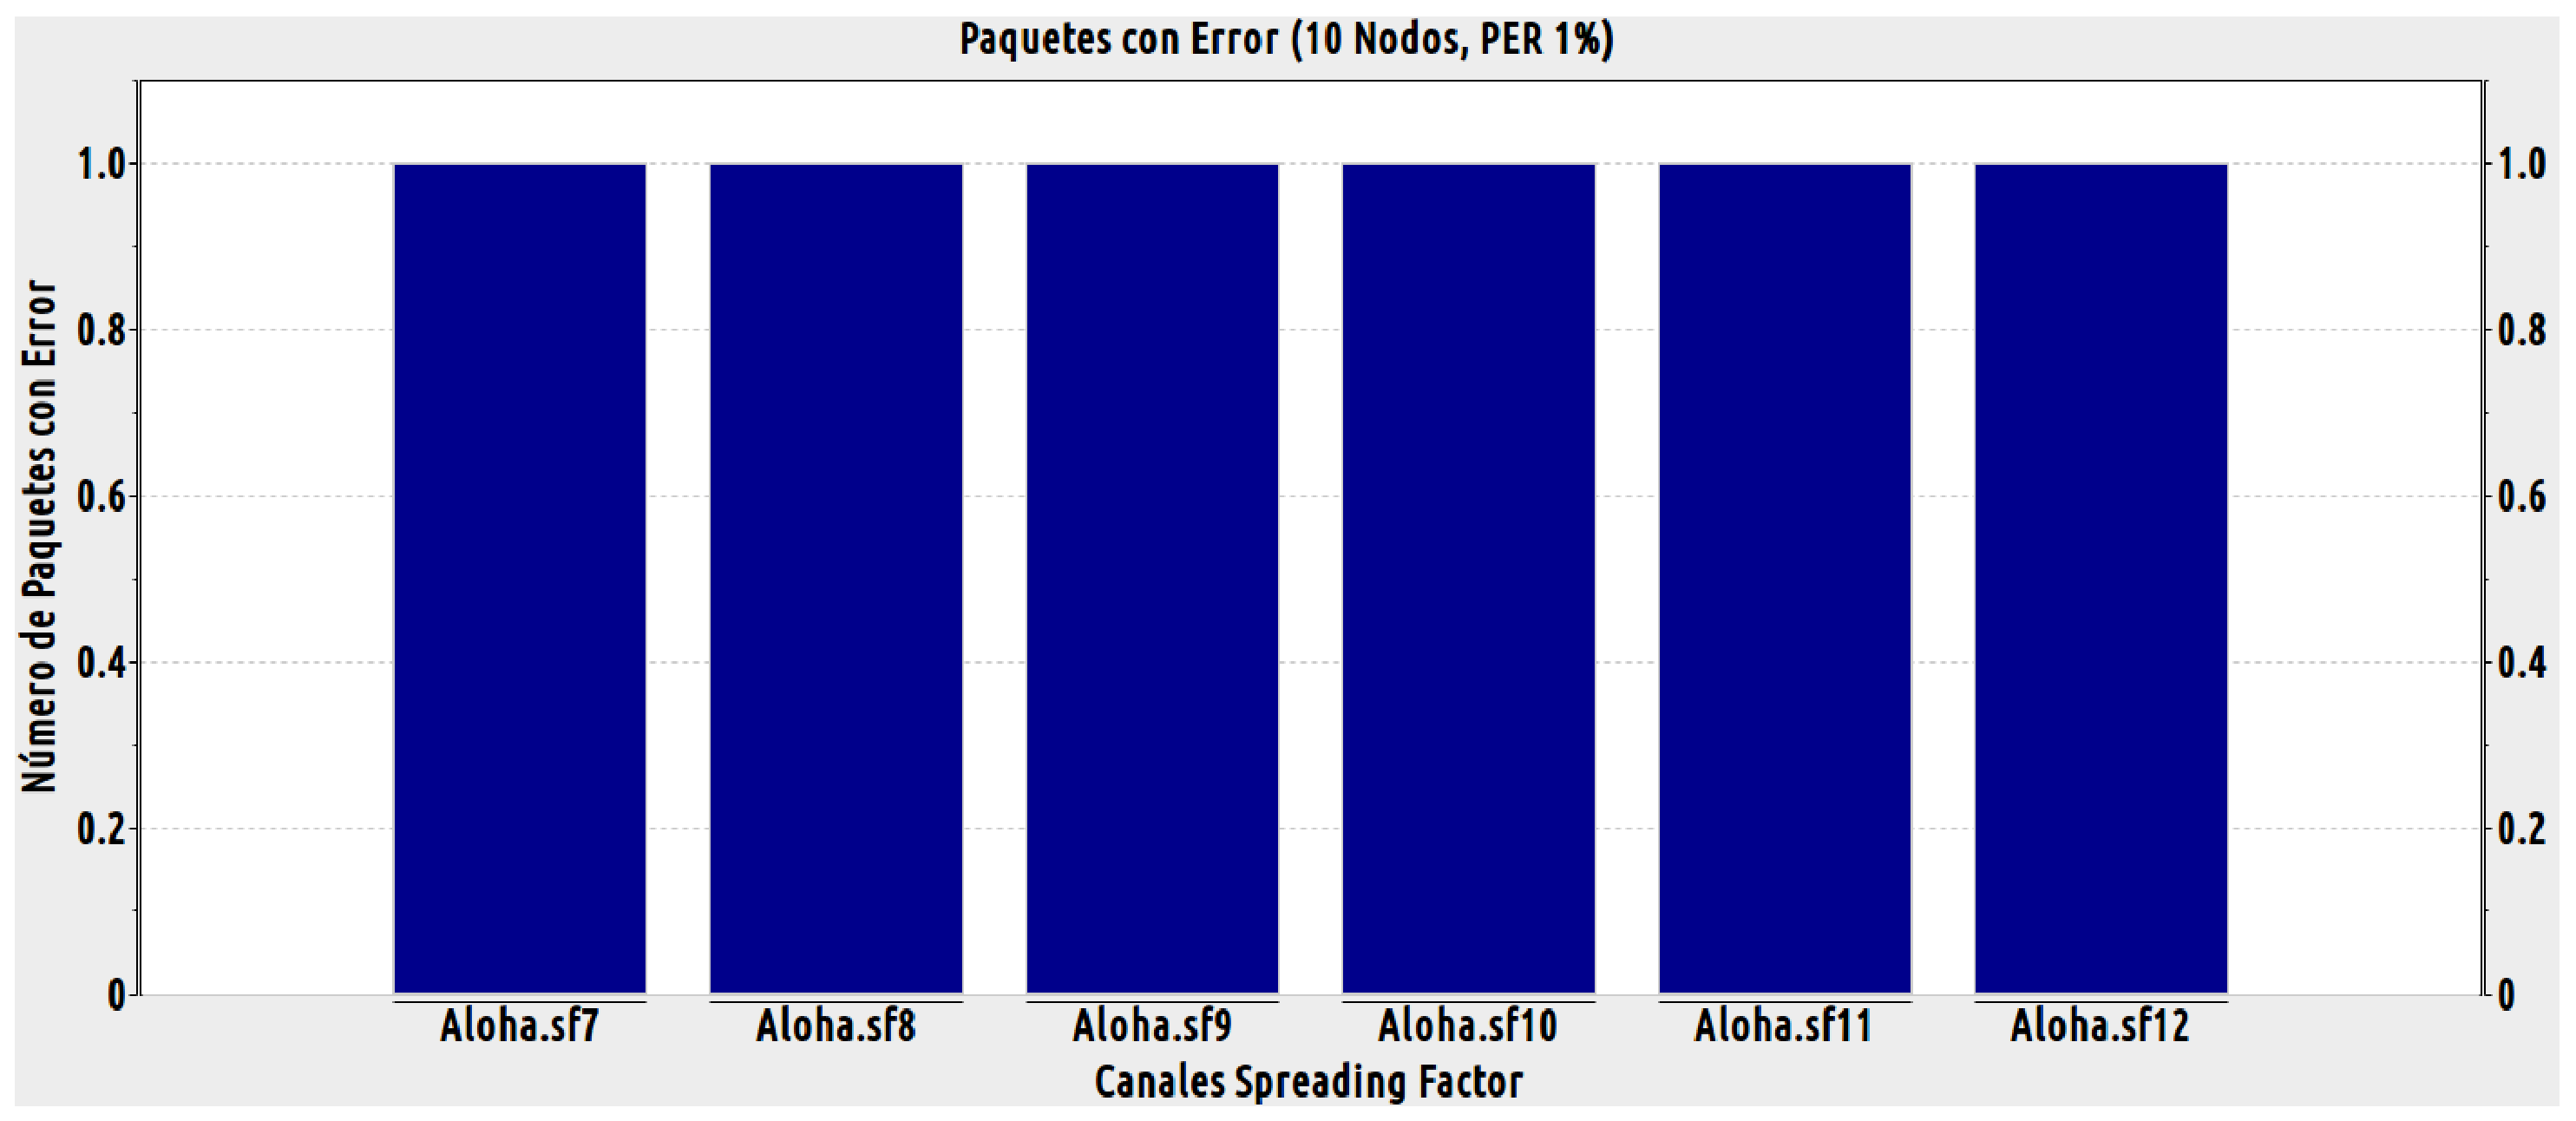
\includegraphics[angle=270, scale=0.4]{images/errores10nodos.eps}
\caption{Gráfico de cantidad de paquetes con errores en cada Spreading Factor en la simulación, para 10 nodos}
\label{anexb:3}
\end{figure}

\begin{figure}[!ht]
\centering
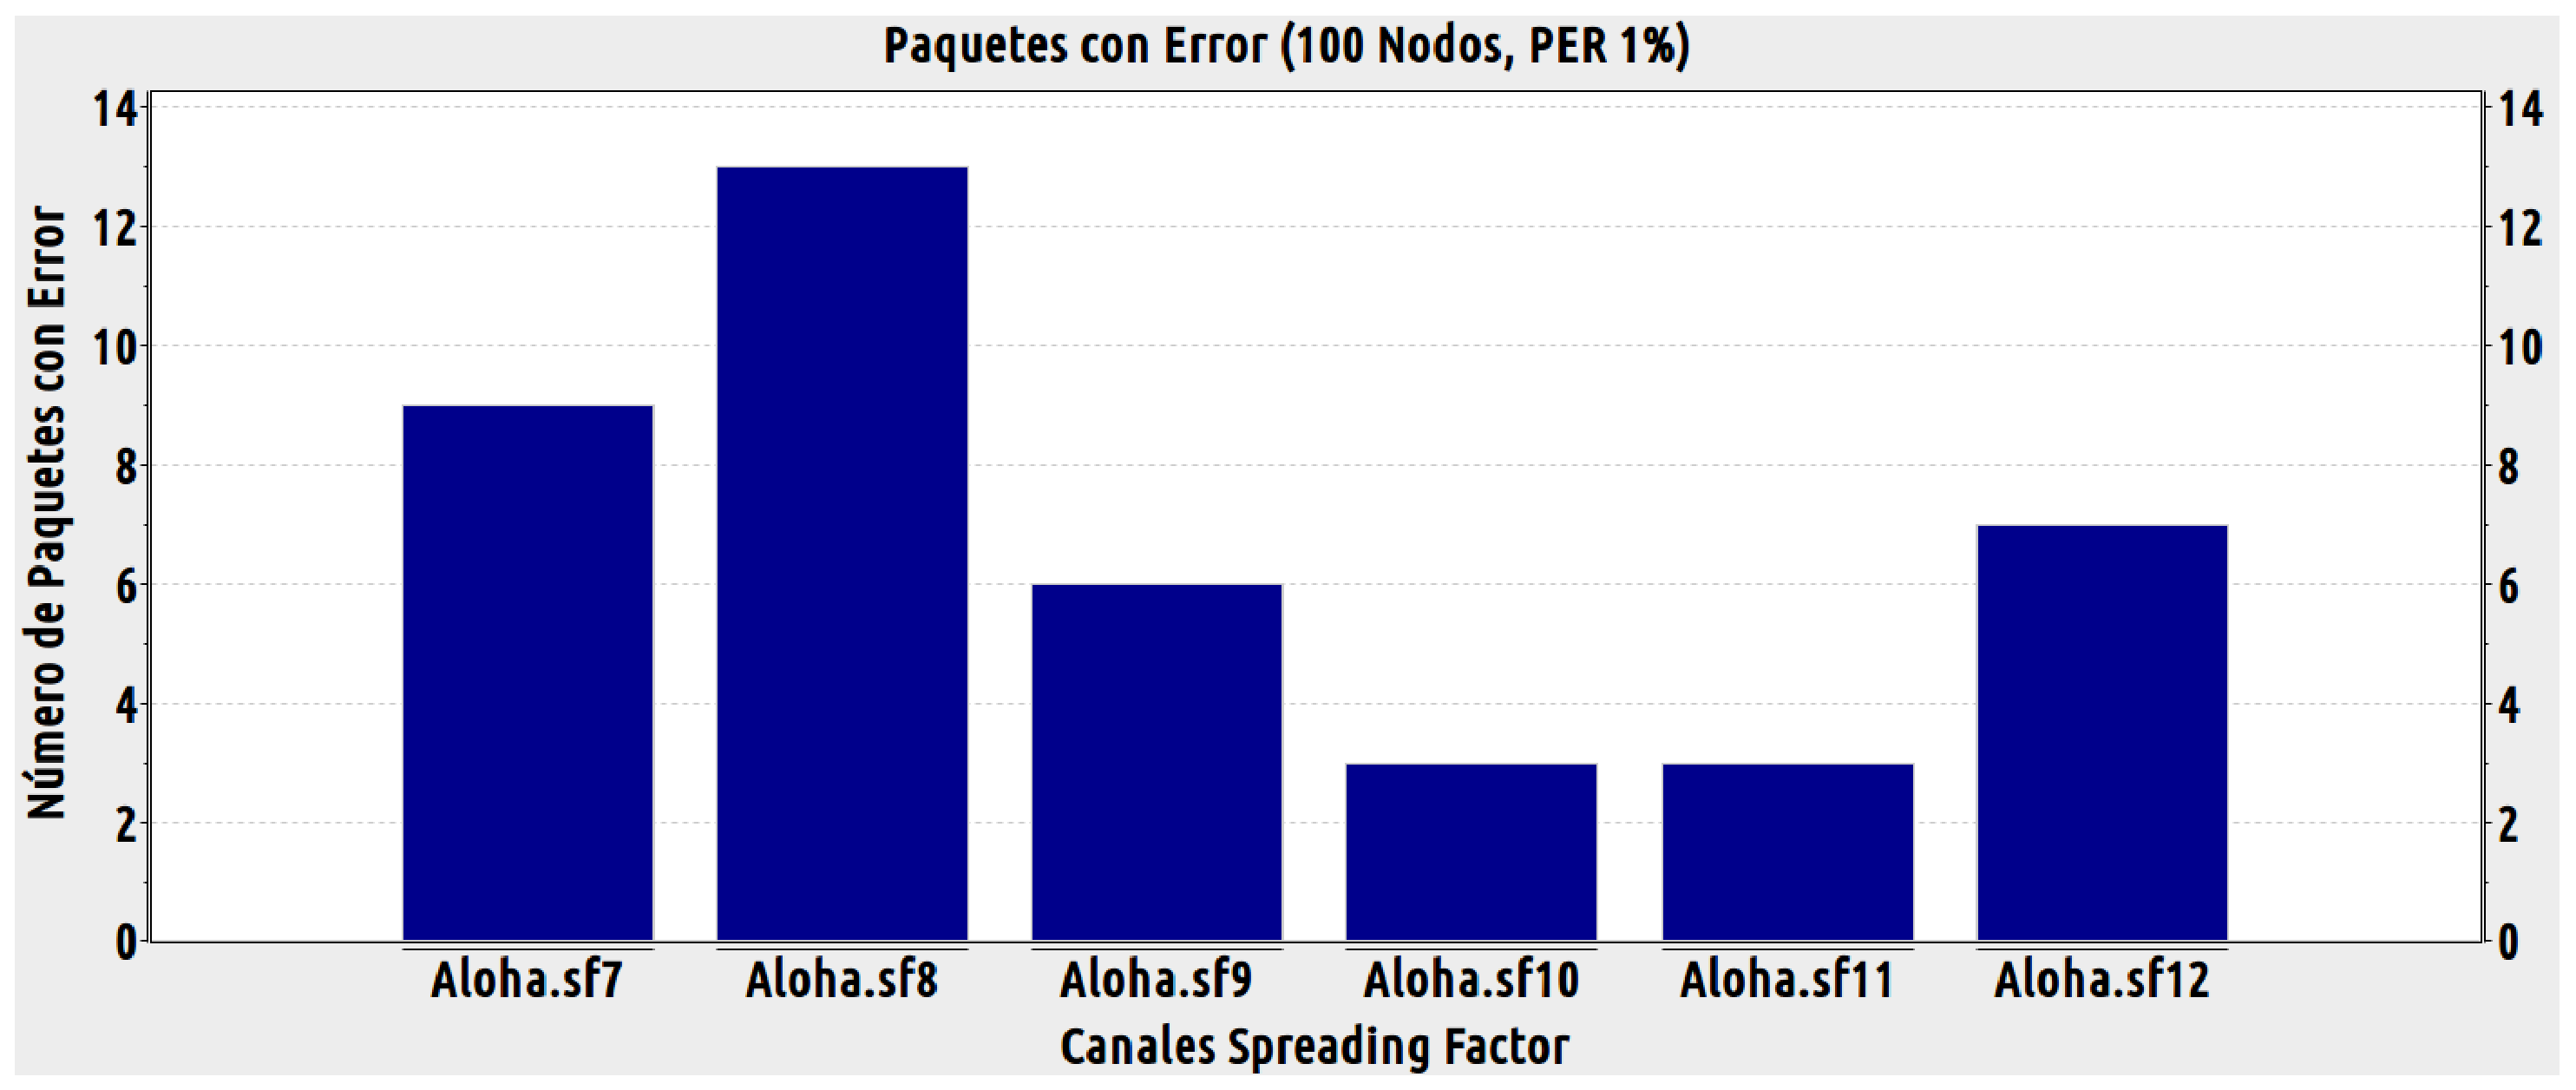
\includegraphics[angle=270, scale=0.4]{images/errores100nodos.eps}
\caption{Gráfico de cantidad de paquetes con errores en cada Spreading Factor en la simulación, para 100 nodos}
\label{anexb:4}
\end{figure}
